\subsection{Организация аппаратного комплекса системы}
\label{sub:system-implementation:hardware}

\FPeval{\NumOfWorkstations}{134}

В соответствии с расположением рабочих станций в отделах и техническими требованиями к системе, а также выбранной клиент-серверной архитектурой разработан аппаратно-технический комплекс системы.

В состав аппаратного-технического комплекса входят:

\begin{itemize}
    \item рабочие места, представленные в виде~\NumOfWorkstations~стационарных компьютеров, подключенных по локальной сети предприятия с помощью модема и коммутаторов;
    \item сервер со специальным программным обеспечением.
\end{itemize}

Аппаратная платформа сервера оптимизирована для нагрузки в 1000~-- 2000 запросов в минуту с упором на экономическую эффективность. Основу серверной инфраструктуры составляют процессоры среднего класса, поддерживающие аппаратную виртуализацию. Подробные требования к аппаратной платформе приведены в таблице~\ref{table:system-implementation:hardware:requirements}.

\begingroup
\singlespacing
\vspace{-\baselineskip}
\begin{longtable}{|>{\raggedright}m{0.2\textwidth}
                  |>{\raggedright}m{0.35\textwidth}
                  |>{\raggedright\arraybackslash}m{0.37\textwidth}|}
    \caption{Требования к аппаратной платформе} \label{table:system-implementation:hardware:requirements} \\ \hline
    Компонент & Минимальные характеристики & Рекомендуемые характеристики \\ \hline
    \endfirsthead
    \multicolumn{3}{@{}l}{\noindent Продолжение таблицы~\thetable} \\ \hline
    Компонент & Минимальные характеристики & Рекомендуемые характеристики \\ \hline
    \endhead
    Процессор & 4 ядра (\textit{Intel Core i5} / \textit{AMD Ryzen 5}) & 8 ядер (\textit{Intel Core i7} / \textit{AMD Ryzen 7}) \\
    \hline
    ОЗУ & 16 ГБ DDR4 & 32 ГБ DDR4 (16 ГБ для \textit{PostgreSQL}) \\
    \hline
    Хранилище & 500 ГБ \textit{SATA} SSD (чтение/запись: 550 МБ/с) & 1 ТБ \textit{NVMe} SSD (чтение/запись: 3500 МБ/с, RAID 1) \\
    \hline
    \textit{Ethernet} & 1 Гбит \textit{Ethernet} & 2×1 Гбит (LACP для балансировки) \\
    \hline
    Видео выход & Интегрированная графика (на базе CPU) & Базовая дискретная видеокарта (для управления) \\
    \hline
    USB порты & 2×USB 3.0 (для периферии/аппаратных ключей) & 4×USB 3.0 (с поддержкой шифрованных носителей) \\
    \hline
    Питание & Блок питания \textit{80+ Bronze} & Блок питания \textit{80+ Platinum} + ИБП 1500VA \\
    \hline
    Уровень шума & <35 дБ (офисное размещение) & <25 дБ (для шумочувствительных зон) \\
    \hline
    Безопасность & TPM 2.0 (опционально) & Аппаратный TPM + поддержка \textit{Secure Boot} \\
    \hline
    Резервное копирование & Внешний NAS (\textit{rsync}) & Ленточный накопитель или облачная \textit{S3}-репликация \\
    \hline
    Поддержи\-ва\-емые ОС & \textit{Ubuntu Server 22.04 LTS} & \textit{RHEL 9} / \textit{Rocky Linux 9} / специализированные дистрибутивы для \textit{Kubernetes} (\textit{k3OS}, \textit{RancherOS}) \\
    \hline
\end{longtable}
\endgroup

Сетевая инфраструктура офисной информационной системы построена с использованием современного аппаратного обеспечения, обеспечивающего стабильную, безопасную и высокоскоростную передачу данных внутри организации. В основе проводной сети лежат управляемые коммутаторы, установленные в распределительном шкафу. Они обеспечивают коммутацию трафика между сегментами сети и поддерживают функции приоритезации трафика (\textit{QoS}), виртуальных локальных сетей (\textit{VLAN}), а также зеркалирования портов для сетевого мониторинга. Все порты коммутаторов рассчитаны на гигабитную скорость передачи данных, что обеспечивает необходимую пропускную способность для офисных приложений.

Маршрутизация и управление доступом к внешним сетям реализованы с помощью выделенного маршрутизатора. Устройство поддерживает механизмы трансляции сетевых адресов (\textit{NAT}), статической и динамической маршрутизации, а также базовые функции межсетевого экранирования. Это обеспечивает надёжное соединение с интернетом и базовую защиту внутренней сети~\cite{book_tanenbaum_computer_networks}.

Для организации беспроводного доступа по всей территории офиса используются точки доступа, подключённые к той же проводной инфраструктуре. Они поддерживают одновременную работу в нескольких диапазонах частот, обеспечивая равномерное покрытие и устойчивую работу мобильных и переносных устройств.

Кабельная система построена на основе экранированной витой пары категории 6, с соблюдением стандартов структурированной кабельной системы. Все коммуникации проложены в скрытых кабель-каналах с выходом в настенные розетки, что обеспечивает как надёжность соединения, так и удобство эксплуатации.

Инфраструктура включает также оборудование для распределения электропитания (\textit{Patch}-панели, стойки, блоки питания с грозозащитой) и систему резервного питания, обеспечивающую бесперебойную работу ключевых сетевых компонентов в случае отключения электроэнергии.

На рис.~\ref{fig:system-implementation:hardware:logical-network} приведена схема логической структуры сети, отражающая принципы организации взаимодействия между основными элементами информационной системы: пользовательскими рабочими станциями, серверными компонентами, сетевым оборудованием и внешними сервисами. 

\begin{figure}[h]
\centering
    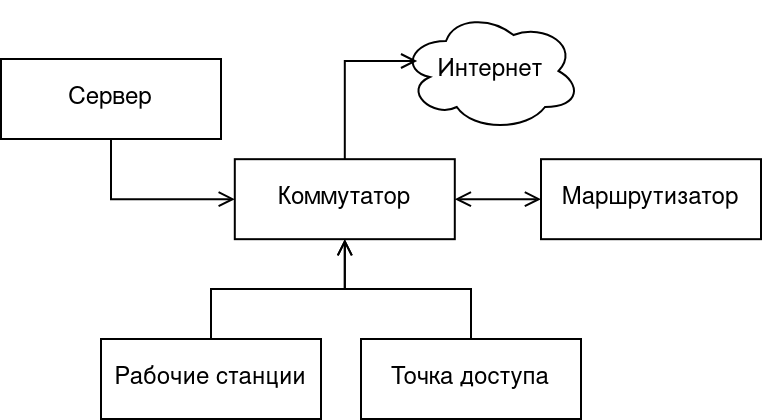
\includegraphics[width=0.8\linewidth]{assets/hardware-logical-network-structure.png}
    \caption{Схема логической структуры сети}
    \label{fig:system-implementation:hardware:logical-network}
\end{figure}

Пользовательский сегмент состоит из офисных рабочих станций, ноутбуков и мобильных устройств сотрудников, подключённых через \textit{Ethernet} или \textit{Wi-Fi}. Все устройства получают IP-адреса по \textit{DHCP} от внутреннего сервера или маршрутизатора. Доступ пользователей к внутренним и внешним ресурсам ограничен политиками безопасности на уровне сетевого шлюза и межсетевого экрана.

Точки доступа \textit{Wi-Fi} (\textit{Access Points}) обеспечивают подключение мобильных устройств и ноутбуков. Поддержка \textit{WPA2/WPA3}, сегментация по \textit{VLAN} и ограничение гостевого доступа применяются для повышения безопасности.

Управляемые коммутаторы (\textit{L2/L3}) объединяют все конечные устройства и серверы, обеспечивая передачу данных по внутренней сети. \textit{VLAN} используются для логического разделения трафика (например, пользователи, серверы, \textit{VoIP}).

Серверный сегмент включает в себя:

\begin{itemize}
    \item веб-сервер, который обслуживает \textit{HTTP/HTTPS}-запросы к системе;
    \item сервер приложений, исполняющий бизнес-логику;
    \item базу данных~-- \textit{PostgreSQL}, работающую в защищённом сегменте без прямого доступа из внешней сети;
    \item файловые хранилища — для обмена и резервного копирования.
\end{itemize}

Между компонентами применяются закрытые соединения по \textit{TCP/IP}, защищённые \textit{TLS} или локальной сетью без выхода наружу.

Внешний трафик, включая обращения к \textit{API} сторонних систем, обновления ПО, а также почтовые и облачные сервисы, направляется через маршрутизатор с \textit{TLS}-шифрованием. \textit{DNS}-запросы и время синхронизируются с доверенными внешними серверами.

Хранилище данных организовано на локальных \textit{SSD} с ежедневным резервным копированием на внешние \textit{NAS} (например, \textit{Synology DS220+}) через \textit{rsync}. Репликация \textit{PostgreSQL} настроена в режиме \textit{master-standby} с асинхронной синхронизацией, что исключает простои при сбоях. Для \textit{Kubernetes Persistent Volumes} используются локальные тома (\textit{LocalPV}), что упрощает управление и снижает затраты на распределенные системы.

Энергоэффективность достигается за счет серверов с блоками питания \textit{80+ Bronze} и настройкой режимов энергосбережения \textit{CPU}. Рекомендуется использование резервного блока питания для защиты от перебоев. Для безопасности используются:

\begin{itemize}
    \item базовый фаервол (\textit{iptables}/\textit{nftables}) с ограничением доступа по \textit{IP} или \textit{MAC}-адресам;
    \item бесплатные \textit{TLS}-сертификаты (\textit{Let’s Encrypt}) для шифрования трафика;
    \item регулярные обновления ОС и ПО через встроенные менеджеры пакетов.
\end{itemize}

Такая конфигурация обеспечивает задержку API-запросов <100 мс. Использование открытого ПО (\textit{Kubernetes}, \textit{PostgreSQL}, \textit{HAProxy}) и стандартного оборудования минимизирует лицензионные расходы, сохраняя гибкость для будущих модернизаций.

Транспортный уровень системы реализован на базе стандартных протоколов, оптимизированных для умеренных нагрузок (1000–2000 \textit{RPM}) и локальной инфраструктуры предприятия. Схема аппаратно-технического комплекса системы представлена на рис.~\ref{fig:system-implementation:hardware:hardware-complex}.

\afterpage{
    \clearpage
    \begin{landscape}
        \thispagestyle{landscape}
        \begin{figure}[p]
            \centering
            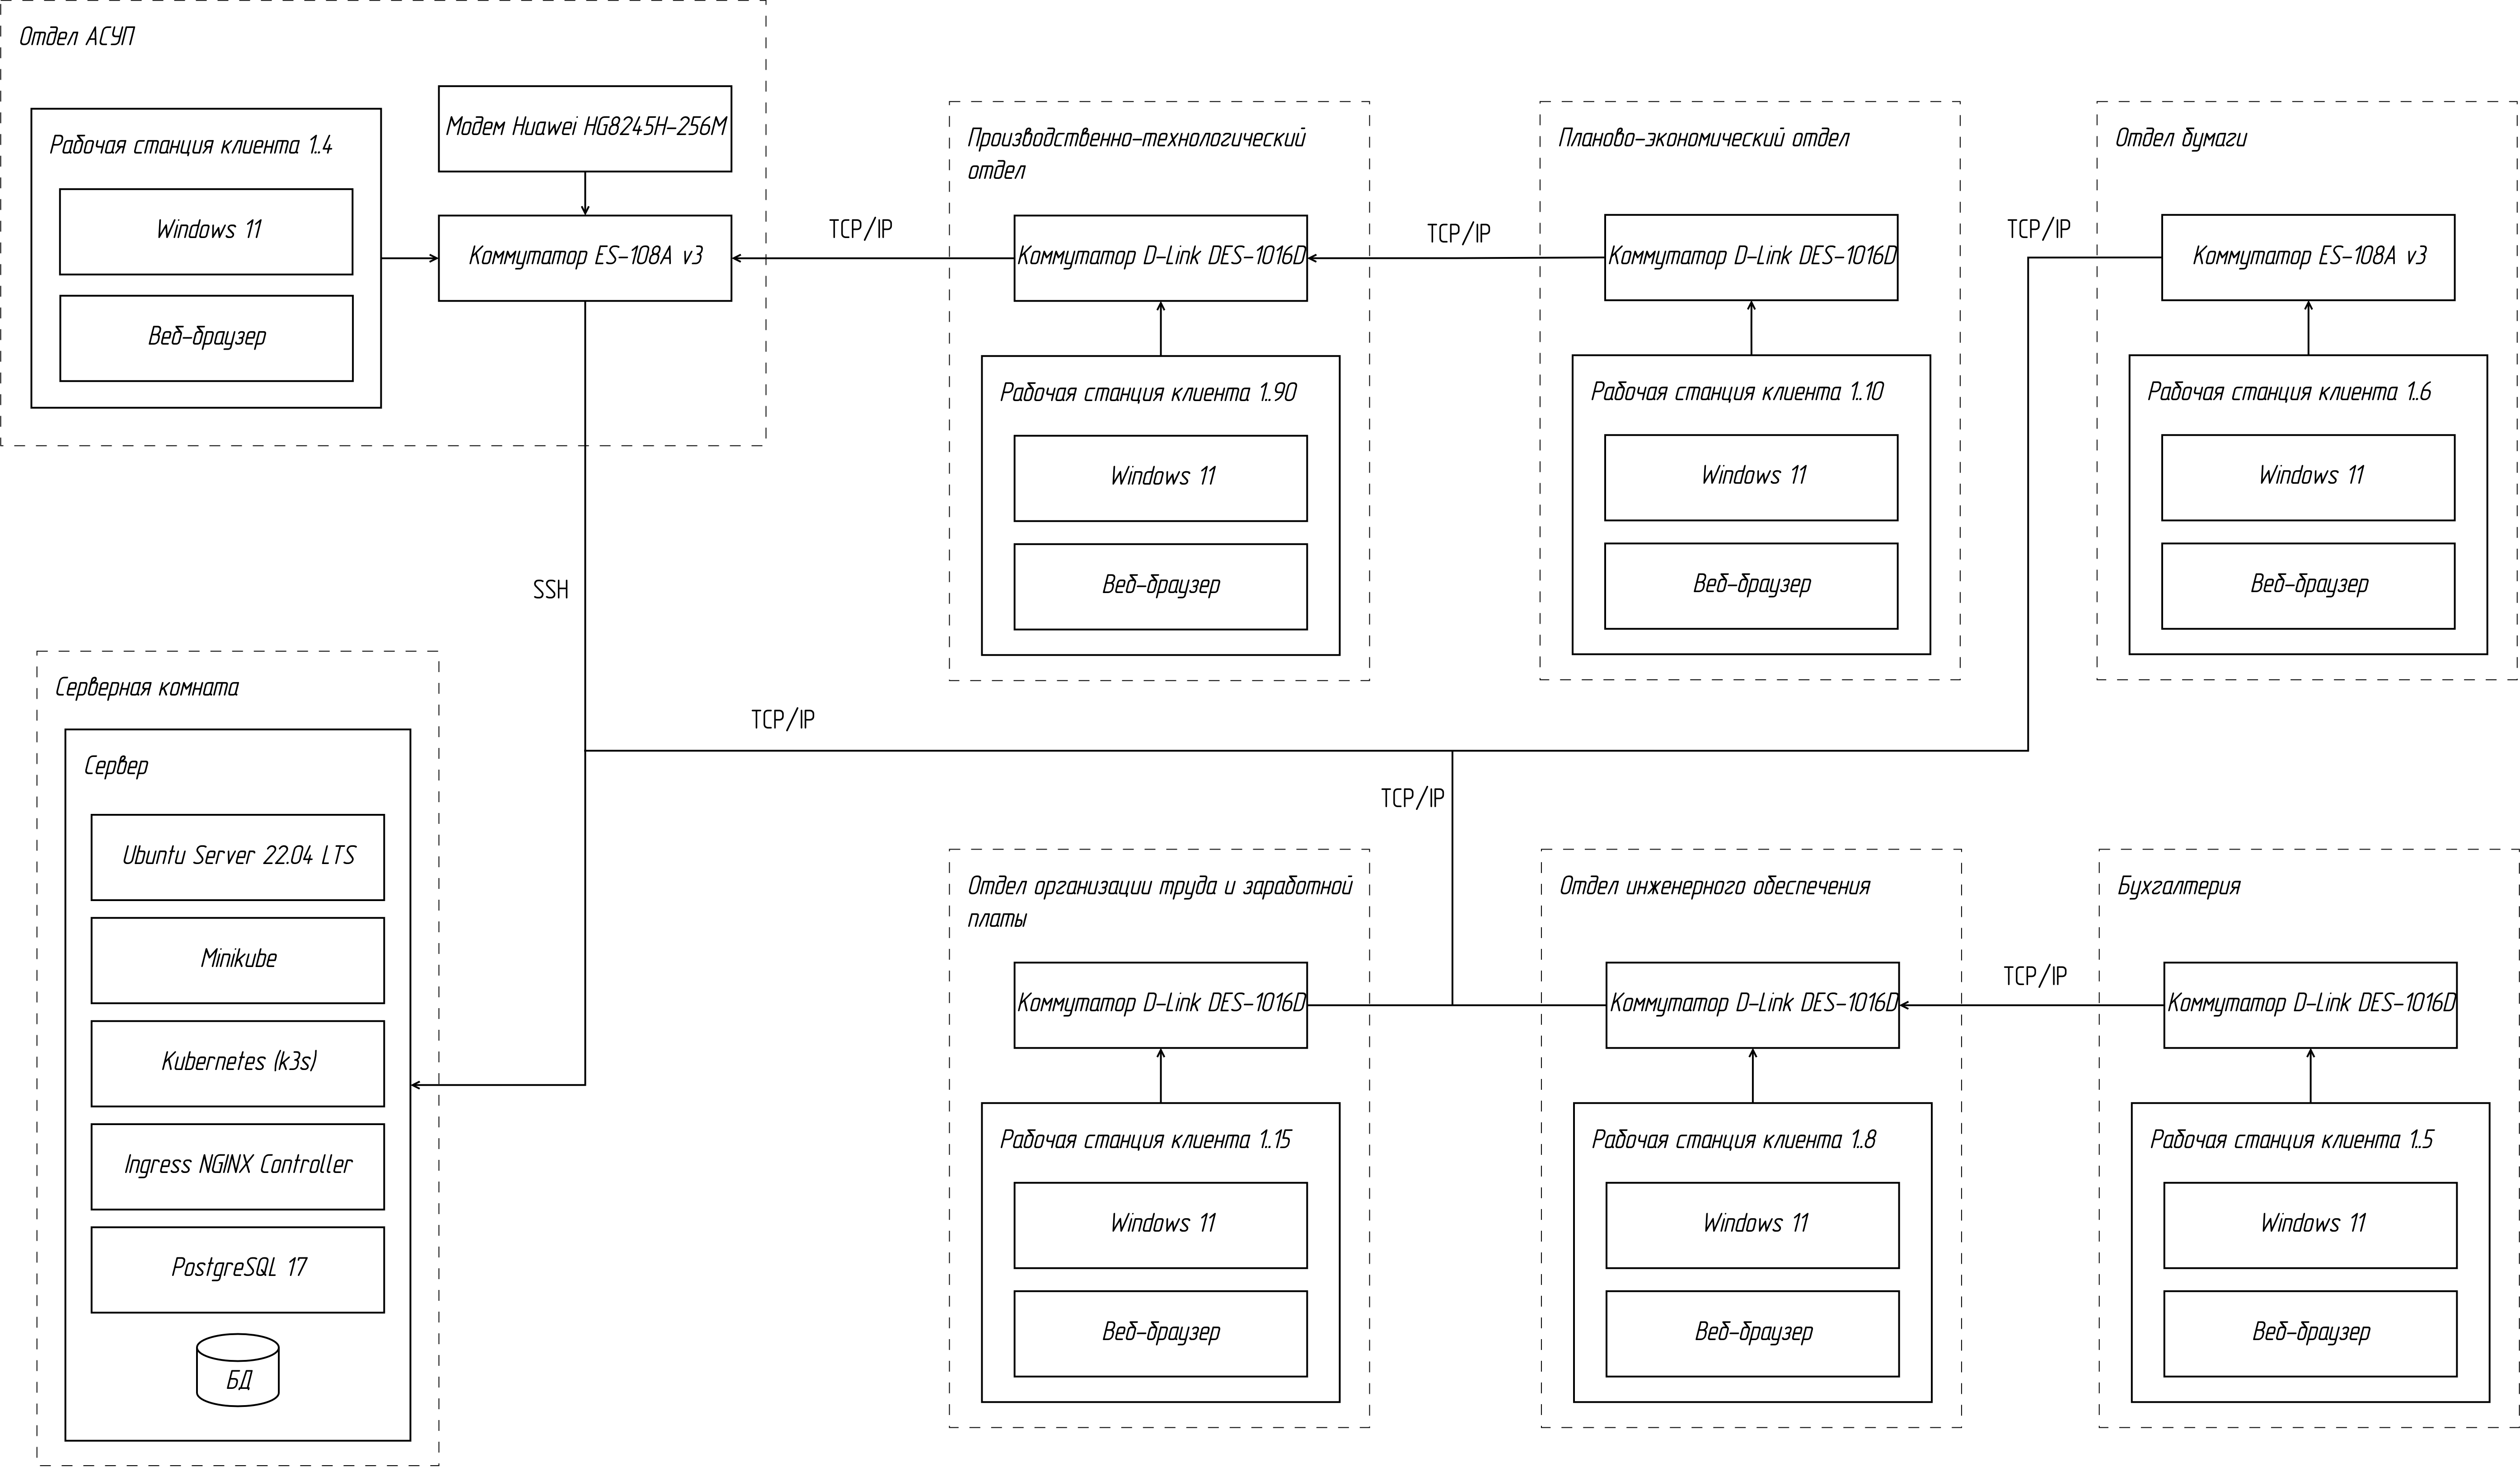
\includegraphics[width=0.99\linewidth]{assets/hardware-complex.png}
            \caption{Схема аппаратно-технического комплекса системы}
            \label{fig:system-implementation:hardware:hardware-complex}
        \end{figure}
    \end{landscape}
    \clearpage
}

\textit{\textbf{Протокол TCP (Transmission Control Protocol)}} обеспечивает надёжную, ориентированную на соединение передачу данных между компонентами системы, что критично для синхронных операций, таких как \textit{HTTP}-запросы к \textit{REST API}, взаимодействие с базой данных PostgreSQL. На уровне установления соединения используется трёхэтапное рукопожатие (\textit{SYN, SYN-ACK, ACK}), гарантирующее согласованность параметров обмена.

После установления соединения \textit{TCP} реализует потоковую передачу данных, разбивая сообщения на сегменты. Каждый сегмент снабжается порядковым номером, что позволяет принимающей стороне упорядочивать полученные данные и обнаруживать пропущенные сегменты. Протокол требует подтверждения получения (\textit{ACK}) для каждого сегмента, и в случае отсутствия подтверждения инициирует повторную передачу, обеспечивая таким образом надёжность доставки.

Протокол \textit{TCP} также включает механизмы управления потоком (\textit{flow control}), основанные на размере окна приёма (\textit{window size}), что позволяет получателю регулировать скорость поступления данных в зависимости от своей обработки. Дополнительно реализовано управление перегрузкой (\textit{congestion control}), позволяющее адаптировать скорость передачи к текущей загрузке сети. На практике это достигается с помощью алгоритмов, таких как \textit{Reno}, \textit{NewReno} или \textit{Cubic}, которые динамически увеличивают или уменьшают размер окна передачи, предотвращая потери данных при перегрузке сети.

Для рассматриваемой системы с нагрузкой 1000–2000 \textit{RPM} ключевыми преимуществами \textit{TCP} являются встроенный механизм повторной передачи потерянных пакетов, автоматическая коррекция порядка доставки и адаптивное управление трафиком, что минимизирует риски потери данных в условиях нестабильного сетевого канала и гарантирует согласованную работу распределённых компонентов.

\textit{\textbf{Протокол AMQP (Advanced Message Quepping Protocol)}} обеспечивает асинхронную коммуникацию между микросервисами через брокер сообщений \textit{RabbitMQ}, реализуя событийно-ориентированную архитектуру рассматриваемой системы. В условиях локальной инфраструктуры \textit{AMQP} работает поверх \textit{TCP}. Это важно для соблюдения гарантий: \textit{TCP} устраняет потерю пакетов, а \textit{AMQP} добавляет уровень логической надежности.

\textit{\textbf{Протокол TLS (Transport Layer Security)}}~-- криптографический протокол, лежащий в основе HTTPS. Процесс шифрования запроса начинается с обмена уникальными сессионными ключами для каждого соединения, что исключает компрометацию прошлых сессий при утечке ключей. После проверки сертификата данные шифруются симметричными алгоритмами. Все внешние \textit{HTTP}-запросы перенаправляются на \textit{HTTPS} с использованием \textit{TLS} 1.3 и сертификатов \textit{Let’s Encrypt}, что защищает данные от перехвата.

Технически, протокол \textit{TLS} работает поверх \textit{TCP} и обеспечивает целостность и конфиденциальность передаваемой информации. Установление соединения происходит через процесс \textit{TLS Handshake}, в ходе которого стороны обмениваются криптографическими параметрами, согласуют алгоритмы шифрования (\textit{cipher suites}) и проводят проверку подлинности с помощью \textit{X.509}-сертификатов. Начиная с версии \textit{TLS} 1.3, протокол существенно упростился: большинство уязвимых и устаревших алгоритмов исключено, \textit{handshake} стал короче (обычно одна \textit{RTT}), а поддержка прямой конфиденциальности (\textit{forward secrecy}) гарантирована использованием протокола обмена ключами \textit{Diffie–Hellman (ECDHE)}.

Шифрование трафика осуществляется симметричными алгоритмами, обеспечивающими высокую скорость работы и стойкость к атаке с подбором. Дополнительно используется \textit{HMAC} (или \textit{AEAD}) для проверки целостности сообщений, предотвращая любые несанкционированные модификации данных в процессе передачи.

На рис.~\ref{fig:system-implementation:hardware:tls-layers-integration} представлена схема слоевой интеграции \textit{TLS} в сетевую модель, иллюстрирующая работу \textit{TLS} в контексте сетевого взаимодействия. \textit{TLS} работает между прикладным и транспортным уровнями: оно шифрует и расшифровывает данные, передаваемые между приложением и \textit{TCP}. \textit{TLS} шифрует только данные приложения. Заголовки \textit{TCP/IP} остаются в открытом виде, чтобы маршрутизаторы могли доставить пакет.

\begin{figure}[h]
\centering
    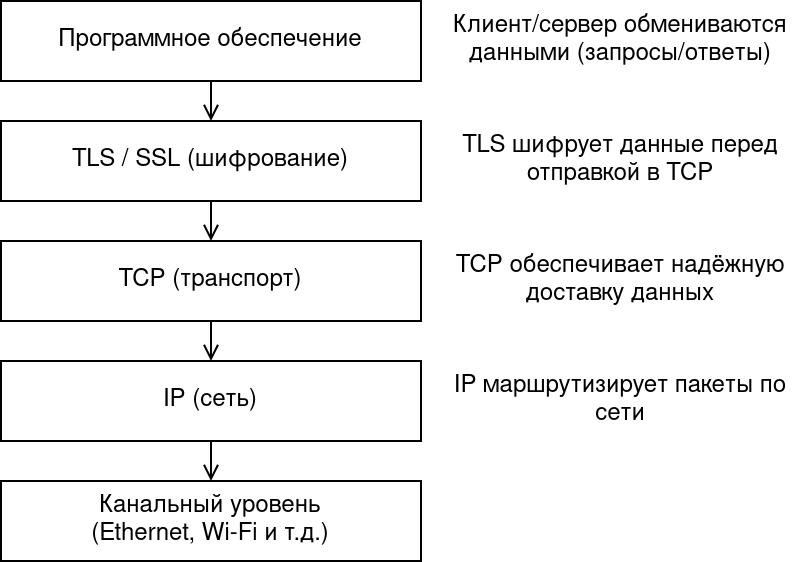
\includegraphics[width=0.7\linewidth]{assets/tls-layers-integration.png}
    \caption{Процесс интеграции \textit{TLS} в сетевую модель взаимодействия}
    \label{fig:system-implementation:hardware:tls-layers-integration}
\end{figure}

\textit{\textbf{Протокол SSH (Secure Shell)}}~-- это криптографический протокол, предназначенный для безопасного удалённого управления операционными системами и передачи данных через незащищённые сети. Работая поверх \textit{TCP} (порт 22 по умолчанию), он обеспечивает полное шифрование трафика, аутентификацию и целостность данных~\cite{book_olifer_network_os}. Используя \textit{SSH} выполняется настройка сервера, конфигурация всех компонентов системы, обновление программного комплекса системы, мониторинг производительности и тд.
